% Source-faithful schematic draft: 2004 Chongqing Science Q12, PDF p.1 (printed p.160).
% Source ID: src-f4f7a5339a68a3cbcf5ef54e4d3736a907b6de9c04c1ef9f3f8b8f7b718d56c4
% Source SHA-256: ef3530a818ad893a36345110d6aa9588de3b793de24c4d6f80333cffa317e429
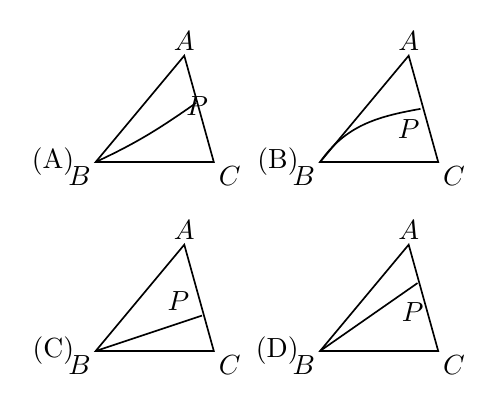
\begin{tikzpicture}[line width=0.6pt, scale=0.75, every node/.style={inner sep=1.5pt}, baseline=(current bounding box.center)]
  % Subfigure (A)
  \begin{scope}[shift={(0, 3.2)}]
    \coordinate (B) at (0, 0);
    \coordinate (C) at (2.0, 0);
    \coordinate (A) at (1.5, 1.8);
    \draw (B) -- (C) -- (A) -- cycle;
    \draw (B) to[out=25, in=215] (1.7, 1.0);
    \node[above] at (A) {$A$};
    \node[below left] at (B) {$B$};
    \node[below right] at (C) {$C$};
    \node[right] at (1.45, 0.95) {$P$};
    \node[left=6pt] at (B) {(A)};
  \end{scope}

  % Subfigure (B)
  \begin{scope}[shift={(3.8, 3.2)}]
    \coordinate (B) at (0, 0);
    \coordinate (C) at (2.0, 0);
    \coordinate (A) at (1.5, 1.8);
    \draw (B) -- (C) -- (A) -- cycle;
    \draw (B) to[out=55, in=190] (1.7, 0.9);
    \node[above] at (A) {$A$};
    \node[below left] at (B) {$B$};
    \node[below right] at (C) {$C$};
    \node[below] at (1.5, 0.8) {$P$};
    \node[left=6pt] at (B) {(B)};
  \end{scope}

  % Subfigure (C)
  \begin{scope}[shift={(0, 0)}]
    \coordinate (B) at (0, 0);
    \coordinate (C) at (2.0, 0);
    \coordinate (A) at (1.5, 1.8);
    \draw (B) -- (C) -- (A) -- cycle;
    \draw (B) -- (1.8, 0.6);
    \node[above] at (A) {$A$};
    \node[below left] at (B) {$B$};
    \node[below right] at (C) {$C$};
    \node[above] at (1.4, 0.6) {$P$};
    \node[left=6pt] at (B) {(C)};
  \end{scope}

  % Subfigure (D)
  \begin{scope}[shift={(3.8, 0)}]
    \coordinate (B) at (0, 0);
    \coordinate (C) at (2.0, 0);
    \coordinate (A) at (1.5, 1.8);
    \draw (B) -- (C) -- (A) -- cycle;
    \draw (B) -- (1.65, 1.15);
    \node[above] at (A) {$A$};
    \node[below left] at (B) {$B$};
    \node[below right] at (C) {$C$};
    \node[below right] at (1.3, 0.9) {$P$};
    \node[left=6pt] at (B) {(D)};
  \end{scope}
\end{tikzpicture}
